\begin{frame}
	\frametitle{Freeciv}

	\begin{itemize}
		\item<1-> Versión \textcolor{UDCpink}{\textit{open source}} y \textcolor{UDCpink}{gratuita} de Sid Meier's Civilization creado en la universidad de Aarhus.
		
		\vspace{1em}
		
		\item<2-> Estrategia por turnos.
		
		\vspace{1em}
		
		\item<3-> El jugador controla a un grupo de colonos en el año 4000 A.C.
		
		\vspace{1em}
		
		\item<4-> Existen 5 formas de finalizar el juego:
		
		\vspace{0.5em}
		
		\begin{itemize}
			\item Victoria por dominación, científica, religión, cultural o por puntuación.
		\end{itemize}
	\end{itemize}
\end{frame}

\begin{frame}
\frametitle{Tipos de terrenos en Freeciv}

\begin{itemize}
	\item<1-> Hay \textcolor{UDCpink}{12 tipos de terreno}, con posible bonificación.
	
	\vspace{1em}
	
	\item<2-> Elementos especiales (lagos, ríos, etc...)
\end{itemize}

\vspace{1em}

\pause[3]

\centering
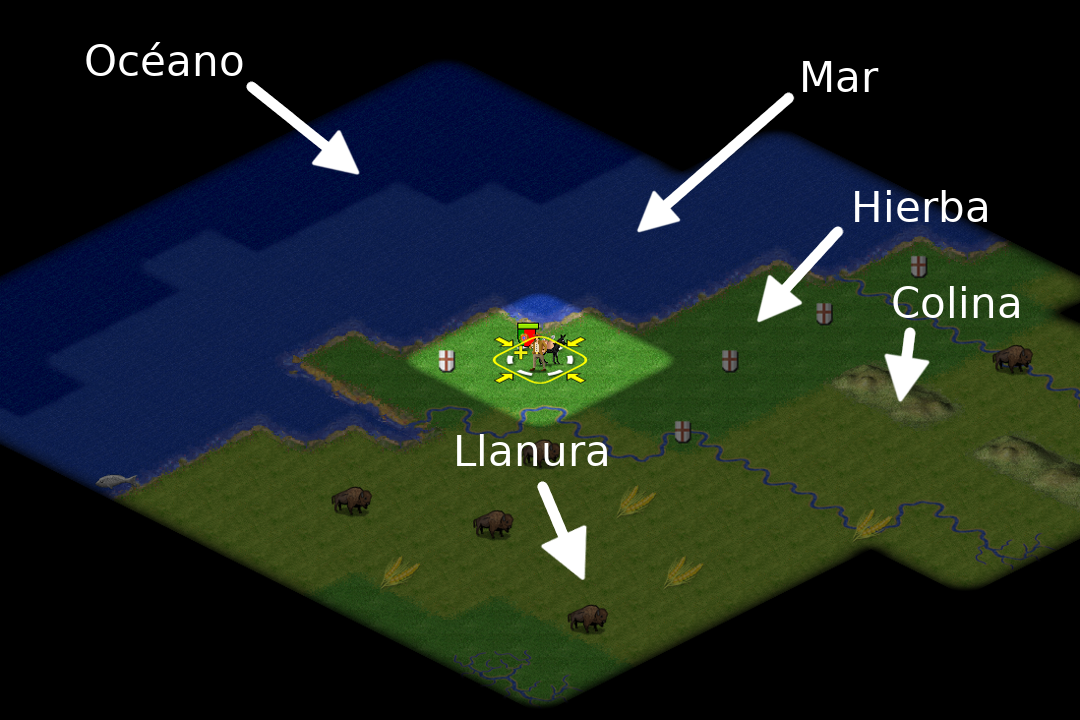
\includegraphics[width=0.5\textwidth]{images/freeciv-example.png}
\end{frame}


\begin{frame}
\frametitle{Objetivos del proyecto}

\begin{itemize}
	\item<1-> Definición de un \textcolor{UDCpink}{modelo declarativo} del escenario usando \textcolor{UDCpink}{\itshape Answer Set Programming}.
	
	\vspace{1em}
	
	\item<2-> Construcción de una pequeña \textcolor{UDCpink}{herramienta gráfica} con la que manipular el escenario.
	
	\vspace{1em}
	
	\item<3-> Eficiencia: reducir o podar el número de combinaciones posibles.
\end{itemize}

\end{frame}
